\PassOptionsToPackage{unicode=true}{hyperref} % options for packages loaded elsewhere
\PassOptionsToPackage{hyphens}{url}
%
\documentclass[]{article}
\usepackage{lmodern}
\usepackage{amssymb,amsmath}
\usepackage{ifxetex,ifluatex}
\usepackage{fixltx2e} % provides \textsubscript
\ifnum 0\ifxetex 1\fi\ifluatex 1\fi=0 % if pdftex
  \usepackage[T1]{fontenc}
  \usepackage[utf8]{inputenc}
  \usepackage{textcomp} % provides euro and other symbols
\else % if luatex or xelatex
  \usepackage{unicode-math}
  \defaultfontfeatures{Ligatures=TeX,Scale=MatchLowercase}
\fi
% use upquote if available, for straight quotes in verbatim environments
\IfFileExists{upquote.sty}{\usepackage{upquote}}{}
% use microtype if available
\IfFileExists{microtype.sty}{%
\usepackage[]{microtype}
\UseMicrotypeSet[protrusion]{basicmath} % disable protrusion for tt fonts
}{}
\IfFileExists{parskip.sty}{%
\usepackage{parskip}
}{% else
\setlength{\parindent}{0pt}
\setlength{\parskip}{6pt plus 2pt minus 1pt}
}
\usepackage{hyperref}
\hypersetup{
            pdfborder={0 0 0},
            breaklinks=true}
\urlstyle{same}  % don't use monospace font for urls
\usepackage[margin=1in]{geometry}
\usepackage{color}
\usepackage{fancyvrb}
\newcommand{\VerbBar}{|}
\newcommand{\VERB}{\Verb[commandchars=\\\{\}]}
\DefineVerbatimEnvironment{Highlighting}{Verbatim}{commandchars=\\\{\}}
% Add ',fontsize=\small' for more characters per line
\usepackage{framed}
\definecolor{shadecolor}{RGB}{248,248,248}
\newenvironment{Shaded}{\begin{snugshade}}{\end{snugshade}}
\newcommand{\AlertTok}[1]{\textcolor[rgb]{0.94,0.16,0.16}{#1}}
\newcommand{\AnnotationTok}[1]{\textcolor[rgb]{0.56,0.35,0.01}{\textbf{\textit{#1}}}}
\newcommand{\AttributeTok}[1]{\textcolor[rgb]{0.77,0.63,0.00}{#1}}
\newcommand{\BaseNTok}[1]{\textcolor[rgb]{0.00,0.00,0.81}{#1}}
\newcommand{\BuiltInTok}[1]{#1}
\newcommand{\CharTok}[1]{\textcolor[rgb]{0.31,0.60,0.02}{#1}}
\newcommand{\CommentTok}[1]{\textcolor[rgb]{0.56,0.35,0.01}{\textit{#1}}}
\newcommand{\CommentVarTok}[1]{\textcolor[rgb]{0.56,0.35,0.01}{\textbf{\textit{#1}}}}
\newcommand{\ConstantTok}[1]{\textcolor[rgb]{0.00,0.00,0.00}{#1}}
\newcommand{\ControlFlowTok}[1]{\textcolor[rgb]{0.13,0.29,0.53}{\textbf{#1}}}
\newcommand{\DataTypeTok}[1]{\textcolor[rgb]{0.13,0.29,0.53}{#1}}
\newcommand{\DecValTok}[1]{\textcolor[rgb]{0.00,0.00,0.81}{#1}}
\newcommand{\DocumentationTok}[1]{\textcolor[rgb]{0.56,0.35,0.01}{\textbf{\textit{#1}}}}
\newcommand{\ErrorTok}[1]{\textcolor[rgb]{0.64,0.00,0.00}{\textbf{#1}}}
\newcommand{\ExtensionTok}[1]{#1}
\newcommand{\FloatTok}[1]{\textcolor[rgb]{0.00,0.00,0.81}{#1}}
\newcommand{\FunctionTok}[1]{\textcolor[rgb]{0.00,0.00,0.00}{#1}}
\newcommand{\ImportTok}[1]{#1}
\newcommand{\InformationTok}[1]{\textcolor[rgb]{0.56,0.35,0.01}{\textbf{\textit{#1}}}}
\newcommand{\KeywordTok}[1]{\textcolor[rgb]{0.13,0.29,0.53}{\textbf{#1}}}
\newcommand{\NormalTok}[1]{#1}
\newcommand{\OperatorTok}[1]{\textcolor[rgb]{0.81,0.36,0.00}{\textbf{#1}}}
\newcommand{\OtherTok}[1]{\textcolor[rgb]{0.56,0.35,0.01}{#1}}
\newcommand{\PreprocessorTok}[1]{\textcolor[rgb]{0.56,0.35,0.01}{\textit{#1}}}
\newcommand{\RegionMarkerTok}[1]{#1}
\newcommand{\SpecialCharTok}[1]{\textcolor[rgb]{0.00,0.00,0.00}{#1}}
\newcommand{\SpecialStringTok}[1]{\textcolor[rgb]{0.31,0.60,0.02}{#1}}
\newcommand{\StringTok}[1]{\textcolor[rgb]{0.31,0.60,0.02}{#1}}
\newcommand{\VariableTok}[1]{\textcolor[rgb]{0.00,0.00,0.00}{#1}}
\newcommand{\VerbatimStringTok}[1]{\textcolor[rgb]{0.31,0.60,0.02}{#1}}
\newcommand{\WarningTok}[1]{\textcolor[rgb]{0.56,0.35,0.01}{\textbf{\textit{#1}}}}
\usepackage{longtable,booktabs}
% Fix footnotes in tables (requires footnote package)
\IfFileExists{footnote.sty}{\usepackage{footnote}\makesavenoteenv{longtable}}{}
\usepackage{graphicx,grffile}
\makeatletter
\def\maxwidth{\ifdim\Gin@nat@width>\linewidth\linewidth\else\Gin@nat@width\fi}
\def\maxheight{\ifdim\Gin@nat@height>\textheight\textheight\else\Gin@nat@height\fi}
\makeatother
% Scale images if necessary, so that they will not overflow the page
% margins by default, and it is still possible to overwrite the defaults
% using explicit options in \includegraphics[width, height, ...]{}
\setkeys{Gin}{width=\maxwidth,height=\maxheight,keepaspectratio}
\setlength{\emergencystretch}{3em}  % prevent overfull lines
\providecommand{\tightlist}{%
  \setlength{\itemsep}{0pt}\setlength{\parskip}{0pt}}
\setcounter{secnumdepth}{0}
% Redefines (sub)paragraphs to behave more like sections
\ifx\paragraph\undefined\else
\let\oldparagraph\paragraph
\renewcommand{\paragraph}[1]{\oldparagraph{#1}\mbox{}}
\fi
\ifx\subparagraph\undefined\else
\let\oldsubparagraph\subparagraph
\renewcommand{\subparagraph}[1]{\oldsubparagraph{#1}\mbox{}}
\fi

% set default figure placement to htbp
\makeatletter
\def\fps@figure{htbp}
\makeatother


\author{}
\date{\vspace{-2.5em}}

\begin{document}

\hypertarget{recap}{%
\section{Recap}\label{recap}}

\hypertarget{sta-326-2.0-programming-and-data-analysis-with-r}{%
\section{STA 326 2.0 Programming and Data Analysis with
R}\label{sta-326-2.0-programming-and-data-analysis-with-r}}

\hypertarget{data-structures}{%
\section{Data structures}\label{data-structures}}

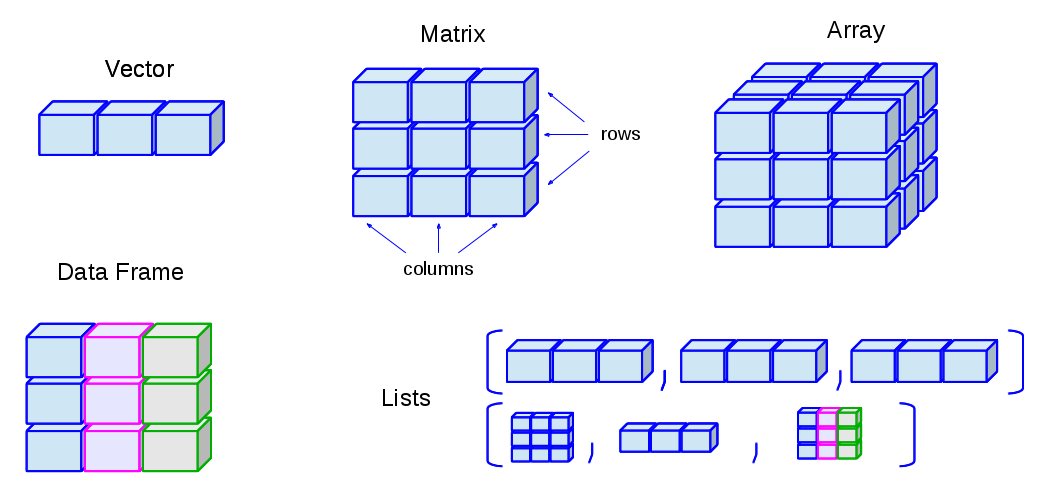
\includegraphics{dataStructures.png}

\begin{itemize}
\item
  Explicit coercion
\item
  Combining objects
\item
  Name elements
\item
  Subsetting
\item
  tibble and factor
\item
  dataframe vs tibble
\item
  Simplifying vector creations
\end{itemize}

\hypertarget{simple-mathematical-and-statistical-functions}{%
\section{Simple mathematical and statistical
functions}\label{simple-mathematical-and-statistical-functions}}

\hypertarget{r-can-be-used-as-a-simple-calculator.}{%
\subsubsection{R can be used as a simple
calculator.}\label{r-can-be-used-as-a-simple-calculator.}}

\begin{longtable}[]{@{}ll@{}}
\toprule
\begin{minipage}[b]{0.47\columnwidth}\raggedright
Operator\strut
\end{minipage} & \begin{minipage}[b]{0.47\columnwidth}\raggedright
Description\strut
\end{minipage}\tabularnewline
\midrule
\endhead
\begin{minipage}[t]{0.47\columnwidth}\raggedright
+\strut
\end{minipage} & \begin{minipage}[t]{0.47\columnwidth}\raggedright
addition\strut
\end{minipage}\tabularnewline
\begin{minipage}[t]{0.47\columnwidth}\raggedright
-\strut
\end{minipage} & \begin{minipage}[t]{0.47\columnwidth}\raggedright
substraction\strut
\end{minipage}\tabularnewline
\begin{minipage}[t]{0.47\columnwidth}\raggedright
*\strut
\end{minipage} & \begin{minipage}[t]{0.47\columnwidth}\raggedright
multiplication\strut
\end{minipage}\tabularnewline
\begin{minipage}[t]{0.47\columnwidth}\raggedright
\^{}\strut
\end{minipage} & \begin{minipage}[t]{0.47\columnwidth}\raggedright
exponentiation (5\^{}2 is 25)\strut
\end{minipage}\tabularnewline
\begin{minipage}[t]{0.47\columnwidth}\raggedright
\%\%\strut
\end{minipage} & \begin{minipage}[t]{0.47\columnwidth}\raggedright
modulo-remainder of the division of the number to the left by the number
on its right. (5\%\%3 is 2)\strut
\end{minipage}\tabularnewline
\bottomrule
\end{longtable}

\hypertarget{some-more-maths-functions}{%
\subsubsection{Some more maths
functions}\label{some-more-maths-functions}}

\begin{longtable}[]{@{}ll@{}}
\toprule
\begin{minipage}[b]{0.47\columnwidth}\raggedright
Operator\strut
\end{minipage} & \begin{minipage}[b]{0.47\columnwidth}\raggedright
Description\strut
\end{minipage}\tabularnewline
\midrule
\endhead
\begin{minipage}[t]{0.47\columnwidth}\raggedright
abs(x)\strut
\end{minipage} & \begin{minipage}[t]{0.47\columnwidth}\raggedright
absolute value of x\strut
\end{minipage}\tabularnewline
\begin{minipage}[t]{0.47\columnwidth}\raggedright
log(x, base=y)\strut
\end{minipage} & \begin{minipage}[t]{0.47\columnwidth}\raggedright
logarithm of x with base y; if base is not specified, returns the
natural logarithm\strut
\end{minipage}\tabularnewline
\begin{minipage}[t]{0.47\columnwidth}\raggedright
exp(x)\strut
\end{minipage} & \begin{minipage}[t]{0.47\columnwidth}\raggedright
exponential of x\strut
\end{minipage}\tabularnewline
\begin{minipage}[t]{0.47\columnwidth}\raggedright
sqrt(x)\strut
\end{minipage} & \begin{minipage}[t]{0.47\columnwidth}\raggedright
square root of x\strut
\end{minipage}\tabularnewline
\begin{minipage}[t]{0.47\columnwidth}\raggedright
factorial(x)\strut
\end{minipage} & \begin{minipage}[t]{0.47\columnwidth}\raggedright
factorial of x\strut
\end{minipage}\tabularnewline
\bottomrule
\end{longtable}

\hypertarget{basic-statistic-functions}{%
\subsubsection{Basic statistic
functions}\label{basic-statistic-functions}}

\begin{longtable}[]{@{}ll@{}}
\toprule
Operator & Description\tabularnewline
\midrule
\endhead
mean(x) & mean of x\tabularnewline
median(x) & median of x\tabularnewline
mode(x) & mode of x\tabularnewline
var(x) & variance of x\tabularnewline
scale(x) & z-score of x\tabularnewline
quantile(x) & quantiles of x\tabularnewline
summary(x) & summary of x: mean, minimum, maximum, etc.\tabularnewline
\bottomrule
\end{longtable}

\hypertarget{probability-distribution-functions}{%
\subsubsection{Probability distribution
functions}\label{probability-distribution-functions}}

\begin{itemize}
\item
  \textbf{d} prefix for the \textbf{distribution} function
\item
  \textbf{p} prefix for the \textbf{cummulative probability}
\item
  \textbf{q} prefix for the \textbf{quantile}
\item
  \textbf{r} prefix for the \textbf{random} number generator
\end{itemize}

\hypertarget{logical-operations}{%
\subsubsection{Logical operations}\label{logical-operations}}

\textbar{}\textless{} \textbar{}less than\textbar{}
\textbar{}\textless{}= \textbar{}less than or equal to\textbar{}
\textbar{}\textgreater{} \textbar{}greater than\textbar{}
\textbar{}\textgreater{}= \textbar{}greater than or equal to\textbar{}
\textbar{}== \textbar{}exactly equal to\textbar{} \textbar{}!=
\textbar{}not equal to \textbar{} \textbar{}!x \textbar{}Not x\textbar{}
\textbar{}x \textbar{} y \textbar{} x OR y\textbar{} \textbar{}x \& y
\textbar{} x AND y\textbar{} \textbar{}isTRUE(x) \textbar{}test if X is
TRUE\textbar{}

\hypertarget{matrix-operations}{%
\subsubsection{Matrix operations}\label{matrix-operations}}

\begin{itemize}
\item
  Matrix multiplication
\item
  Transpose
\item
  ets
\end{itemize}

\hypertarget{handling-missing-observations}{%
\subsubsection{Handling missing
observations}\label{handling-missing-observations}}

\begin{Shaded}
\begin{Highlighting}[]
\NormalTok{is.na}
\end{Highlighting}
\end{Shaded}

\hypertarget{writing-functions-with-r}{%
\section{Writing functions with R}\label{writing-functions-with-r}}

\begin{Shaded}
\begin{Highlighting}[]
\NormalTok{function_name <-}\StringTok{ }\ControlFlowTok{function}\NormalTok{(inputs)\{}

\OperatorTok{<}\NormalTok{FUNCTION BODY}\OperatorTok{>}

\NormalTok{\}}
\end{Highlighting}
\end{Shaded}

\hypertarget{programming-styles}{%
\section{Programming styles}\label{programming-styles}}

\begin{itemize}
\item
  base R
\item
  tidyverse
\item
  pipe operator \%\textgreater{}\%
\end{itemize}

\hypertarget{import-and-export-data}{%
\section{Import and Export data}\label{import-and-export-data}}

\begin{itemize}
\tightlist
\item
  readr functions
\end{itemize}

\hypertarget{data-visualization}{%
\section{Data Visualization}\label{data-visualization}}

\begin{itemize}
\item
  qplot
\item
  ggplot
\end{itemize}

\hypertarget{data-transform-and-data-wrangling}{%
\section{Data Transform and Data
Wrangling}\label{data-transform-and-data-wrangling}}

\begin{itemize}
\tightlist
\item
  \texttt{tidyr} and \texttt{dplyr} functions
\end{itemize}

\hypertarget{reproducible-reporting}{%
\section{Reproducible reporting}\label{reproducible-reporting}}

\begin{itemize}
\tightlist
\item
  Rmarkdown
\end{itemize}

\hypertarget{random-number-generation}{%
\section{Random number generation}\label{random-number-generation}}

\begin{itemize}
\item
  buil-in functions in R
\item
  Inverse transform method
\end{itemize}

\hypertarget{statistical-modelling-and-inference}{%
\section{Statistical modelling and
Inference}\label{statistical-modelling-and-inference}}

\begin{itemize}
\item
  Regression analysis
\item
  Hypotheses testing
\end{itemize}

\hypertarget{functionals}{%
\section{Functionals}\label{functionals}}

\begin{itemize}
\item
  lapply and sapply
\item
  map
\item
  modify
\item
  map\_df
\end{itemize}

YOUR TURN: Update this with all the topics we discussed.

\end{document}
